\section{Introduzione}
\subsection{Premessa}
In questo capitolo di introduzione verranno utilizzate le idee proposte da un certo Brooks. Non si tratta di verità assolute ma di una buona base per la discussione. In questo corso le opinioni sono più importanti dei fatti.\newline
La notorietà di Brooks è dovuta al suo libro "The Mythical Man-Month". Uno degli argomenti proposti noto come \textbf{Legge di Brooks} afferma che "adding people to a late software project just makes it later".
\subsubsection{Il mito del garage}
Alcune aziende di successo hanno avuto inizio in un garage.\newline
Brooks guardando questi esempi negli anni '70 e si chiedeva "perché non rimpiazzare i grandi team? Non possiamo prendere due o tre persone e metterle in un garage per far funzionare le cose?"\newline
Il problema è che pochi utenti non bastano una volta che il sistema scala. I software scritti in un garage non hanno richiesto approfondite analisi dei requisiti, test, piani di manutenzione, documentazione dettagliata etc.
\paragraph{Apple}
Steve Jobs e Steve Wozniak hanno creato in un garage il primo Apple computer. Tuttavia non è possibile considerare il risultato un "prodotto". Ciò che è stato realizzato nel garage è stato un prototipo, ovvero qualcosa che potesse dimostrare la realizzabilità. Organizzare il processo di produzione e di vendita non è possibile per due persone, perché risulterebbe troppo complessa e ci sono molte casistiche da considerare.\newline
Per esempio una volta che il prodotto arriva nelle case degli utenti deve funzionare bene e non deve richiedere manutenzioni continue.
\paragraph{Google}
Anche Google è iniziata in un garage. Ciò che è uscito è stata la prima interfaccia del motore di ricerca. Perché Google ha avuto successo? Si può pensare che non esistevano ancora motori di ricerca, ma invece esistevano eccome.\newline
Google a differenza di altri però:
\begin{itemize}
	\item Funzionava meglio grazie al suo algoritmo chiamato "PageRank";
	\item Aveva un modello di Business innovativo, valorizzando il dato invece che utilizzare pubblicità. Chi pagava Google veniva privilegiato apparendo prima tra i risultati;
	\item Era semplice da utilizzare, focalizzato sul servizio che erogava;
	\item Aveva idee chiare e si è subito focalizzato sull'infrastruttura e a realizzarla; la "velocità di esecuzione" infatti è spesso più importante dell'idea.
\end{itemize}
\paragraph{Facebook}
Nato da un campus, l'idea era realizzare un'applicazione per scegliere chi fosse più "sexy" tra due compagni di campus. Il problema di Facebook è sempre stata l'infrastruttura, che deve essere molto grande, resistente a malfunzionamenti e fruibile, ma allo stesso tempo deve fruttare denaro. Facebook usa le ad: al momento infatti il suo modello di business è focalizzato per il 98.3\% sulla pubblicità. Il modello è rischioso perché se un giorno i modelli di business cambiassero e la pubblicità sparisse la situazione per FB sarebbe disastrosa.\newline\newline
In conclusione in garage possono nascere buone idee e buoni prototipi, ma non prodotti. Per portare sul mercato un prodotto è necessario fare un piano.
\subsection{Goal, Progetto e Tar Pit}
\subsubsection{Goal}
Una start-up che cerca finanziatori deve avere un modello di business convincente.
$$ GOAL \xrightarrow{} PROGETTO $$
Gli elementi fondamentali sono il \textbf{goal}, che definisce cosa deve essere fatto e il \textbf{progetto} che consentirà  di raggiungere il risultato atteso. La definizione del goal fa parte del progetto.\newline
Il progetto richiede un’attenta gestione per garantire il rispetto del goal, far fronte ai cambiamenti e alla complessità, impiegare “bene” le risorse disponibili (tempo, denaro), organizzare e dirigere il team, le comunicazioni, la documentazione etc.\newline Per portare a termine un progetto è necessario svolgere un’approfondita analisi dei requisiti e dell’architettura, produrre una documentazione dettagliata, etc.
\subsubsection{Cambiamento}
Secondo Brooks bisogna attenersi rigidamente al piano di analisi. Oggi questa visione è piuttosto datata. Tuttavia anche Brooks pensa che il cambiamento sia una costante. Oggi esistono approcci progettuali che non impongono un'analisi troppo dettagliata o vincolante (agile) perché si assume a priori che ci saranno cambiamenti. In questo caso un requisito aggiuntivo è proprio il fatto che \textit{i requisiti possono cambiare, il progetto deve essere abbastanza flessibile da accogliere i cambiamenti}. Il rischio dell'AGILE è però di non convergere mai. Se non si riesce ad arrivare ad un risultato ben definito si rischia di andare avanti all'infinito consumando risorse etc.\newline
Non esistono piani ottimi per affrontare il cambiamento, ma esistono buoni piani, ovvero best practice consigliate. Si cerca di organizzare il progetto per poter riuscire ad utilizzare le risorse nel modo più efficiente possibile.\newline
Il rischio del cambiamento porta alla \textit{tar pit} (sostanzialmente simili alle sabbie mobili). La metafora porta a pensare che nel momento in cui cerchiamo di affrontare il cambiamento panicando/sotto stress si rischia solo di rimanere ancora più impantanati.\newline
L'immagine seguente mostra il livello dello stress legato alle prestazioni in un progetto mano a mano che il tempo avanza.

\centeredImage{document/img/stresscurve.PNG}{Curva dello Stress}{0.5}
\noindent In questa vengono invece visualizzate le fasi classiche di come si affronta il cambiamento. Per esempio quando il cliente ci dice "Questo non è ciò che ho chiesto".
\centeredImage{document/img/changecurve.PNG}{Curva di Kübler-Ross}{0.6}
\noindent In questo caso l'importante è non fermarsi alla fase di "Denial", perché rischiamo di rendere insoddisfatto il cliente e pure di finire in tribunale.
\subsection{Complessità}
La complessità dei progetti è il motivo per cui non si può affidare tutto il lavoro a due sole persone. Solitamente due persone in un garage producono un \textbf{Programma} ovvero un insieme di istruzioni che implementano una o più funzionalità. Scrivere un programma NON equivale a realizzare un prodotto. Progetti molto complessi non si possono suddividere in tanti task indipendenti, è necessaria la comunicazione tra gli sviluppatori, dato che esistono numerose interrelazioni tra i task.\newline
Un \textbf{Prodotto} è più di un programma, è sicuramente molto più oneroso.
Un \textbf{Sistema} è un insieme di componenti o prodotti che interagiscono tra loro per supportare dei processi complessi. Un sistema per essere tale deve:
\begin{itemize}
	\item Definire con precisione le modalità di integrazione tra i componenti;
	\item Definizione dei tracciati (interfacce di comunicazione tra i componenti);
	\item Definizione dei Test;
	\item Utilizzo corretto delle risorse, spesso limitate.
\end{itemize}
Il fattore moltiplicativo non trascurabile di differenza tra prodotto e sistema e circa di 3 volte.\newline
Esistono due tipi di complessità secondo Brooks:
\begin{itemize}
	\item \textbf{Accidental complexity}: riguarda aspetti relativi alle tecnologie impiegate. Si tratta di una complessità che può essere ridotta, per esempio migliorando le tecnologie.
	\item \textbf{Essential complexity}: Riguarda il problema per cui bisogna realizzare il sistema. Questa complessità è difficile da ridurre. Per esempio se un problema è NP, non si può risolvere in tempo polinomiale, al massimo possiamo gestire il problema in modi diversi.
\end{itemize}
Lo scopo del Project Management è cercare di ridurre la Accidental complexity e gestire la Essential complexity.\newline
Una domanda fondamentale che si pone Brooks è: "Perché un progetto fallisce? (Why does software fails?)"\newline
Rispondendo a questa domanda possiamo affrontare meglio il problema. Ma cosa significa fallire? Per esempio se utilizziamo troppe risorse e andiamo in rosso, se il progetto non aderisce alle specifiche o se non rispetta le deadline.\newline
Un progetto fallisce per più motivi, questi sono alcuni dei più comuni:
\begin{itemize}
	\item Non si rispettano gli obiettivi;
	\item Non si stimano correttamente i tempi;
	\item Troppo ottimismo;
	\item Convinzione che basti l'impegno per raggiungere gli obiettivi (Effort $\neq$ Progress);
	\item Mancato monitoraggio dello stato di avanzamento;
	\item Ritardi dovuti all'aggiunta di personale al progetto (dovuti alla formazione).
\end{itemize}
Il processo creativo secondo Dorothy Sayers si divide in tre fasi:
\begin{itemize}
	\item Idea;
	\item Implementazione;
	\item Interazione.
\end{itemize}
Gli sviluppatori sono ottimisti, pensano che tutto andrà sempre bene, ma i problemi emergono durante l'implementazione e l'interazione con gli utenti.
\subsection{The Mythical Man Month}
La probabilità che vada tutto bene è prossima allo zero.
Il semplice uso del man month (mese uomo) come misura delle risorse è sbagliato e pericoloso. Questo perché ogni sviluppatore ha tempi di lavoro e ritmi diversi. La vera domanda da farsi quando si parla di mesi uomo è "a qualche figura professionale hai associato questa misura? Un senior? Junior?".
Inoltre aumentare il personale non fa diminuire lineramente il tempo necessario per porre fine al progetto (avere personale doppio non ridurrà di metà il tempo necessario).\newline
La \textbf{Legge di Masson} dice che "esiste un tempo minimo di sviluppo che non può essere ridotto ulteriormente, anche aumentando le risorse disponibili."
\begin{info}[Esempio]
	In un pit-stop di una Formula 1 (dove si cambiano le gomme consumate, la regolazione degli alettoni etc.). Per ora concentriamoci sul cambio delle gomme. Ci concentriamo sul cambio gomme perché si tratta dell'attività critica, che richiede cioè più tempo. Chi cambia le gomme ha più responsabilità.
	\begin{itemize}
		\item Se avessimo un solo meccanico il cambio delle gomme impiegherebbe tempo \textit{T};
		\item Come si ridurrebbe il tempi di \textit{T}? Dipende dalle strategie utilizzate! Posso aspettarmi di dimezzare il tempo? Circa, al massimo c'è un po' di overhead;
		\item Se ne avessimo 3 non riusciamo ad ottenere un tempo di circa $\frac{T}{3}$.
		\item Con 4 però sembra che il tempo sia in grado di andare vicino a $\frac{T}{4}$, sembra una stima ideale;
		\item Con 8? Riusciamo ad ottenere $\frac{T}{8}$? No...
	\end{itemize}
	Come si può intuire la funzione (numero di personale - tempo) non è affatto lineare.
	Un'ulteriore misura da tenere in considerazione è il costo. Più personale utilizziamo più dobbiamo pagare.\newline
	In questo caso però il tempo ha molto più valore dei costi!\newline
	Ogni meccanico inoltre ha un ruolo bel preciso.
\end{info}
Ci sono diversi scenari e diverse esigenze:
\begin{figure}[H]
	\centering
	\begin{subfigure}{.24\textwidth}
		\centering
		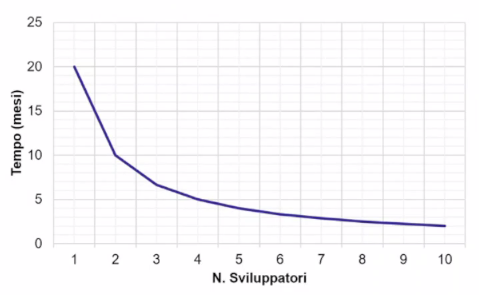
\includegraphics[width=\linewidth]{document/img/noint.PNG}
		\caption{Caso di task perfettamente partizionabili}
	\end{subfigure}%
	\begin{subfigure}{.24\textwidth}
		\centering
		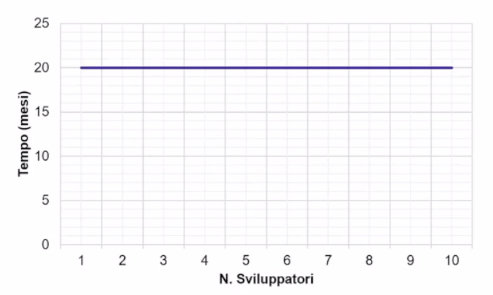
\includegraphics[width=\linewidth]{document/img/nopart.PNG}
		\caption{Caso di task non partizionabili}
	\end{subfigure}%
	\begin{subfigure}{.24\textwidth}
		\centering
		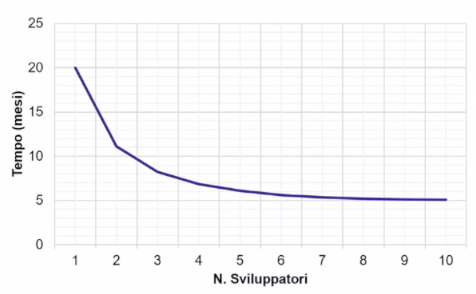
\includegraphics[width=\linewidth]{document/img/comu.PNG}
		\caption{Caso di task che richiedono comunicazioni}
	\end{subfigure}
	\begin{subfigure}{.24\textwidth}
		\centering
		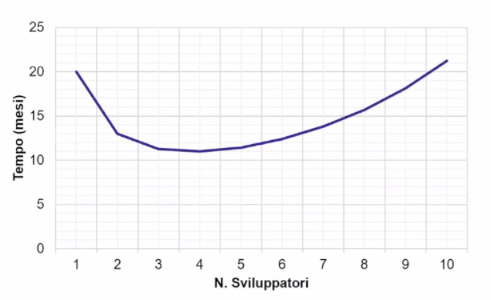
\includegraphics[width=\linewidth]{document/img/nocom.PNG}
		\caption{Caso di task che richiedono complesse interrelazioni}
	\end{subfigure}
\end{figure}
\noindent Notiamo che esistono casi in cui l'aumento di personale può essere addirittura controproducente.\newline\newline
Brooks suggerisce che il tempo complessivo di sviluppo si divide nel seguente modo:
\begin{itemize}
	\item $\frac{1}{3}$: progettazione e pianificazione;
	\item $\frac{1}{6}$: implementazione (scrittura del codice);
	\item $\frac{1}{4}$: test dei componenti (early system test);
	\item $\frac{1}{4}$: test del sistema quando i componenti sono integrati.
\end{itemize}
La scrittura dei test può superare la scrittura delle funzionalità.\newline\newline
Spesso le stime dei tempi sono sbagliate per la \textbf{mancanza di coraggio (gutless estimating)} da parte degli sviluppatori di contrastare le richieste dei manager. I ritardi finali sono i peggiori e i più difficili da affrontare, perché rischiano di mandare nel panico o in depressione gli sviluppatori, che risulteranno quindi meno produttivi.\newline
Quando si riscontra un ritardo è necessario \textbf{modificare il progetto}.\newline
Supponiamo di avere un progetto suddiviso in quattro milestone, ciascuna delle quali dovrà essere portata a termine dopo un mese, utilizzando 3 persone. Una strategia che può utilizzare l'azienda è fare uno shift di un mese per tutte le milestone. Ci sono però alcuni problemi:
\begin{itemize}
	\item Non si investiga su cosa ha portato ritardo, questo può essere causa di replicazione degli stessi errori in futuro;
	\item Se la prima milestone è stata terminata in ritardo ci sono validi motivi per sospettare che forse anche per le prossime potrebbe avere lo stesso destino;
	\item Le deadline potrebbero andare in conflitto con altri progetti dell'azienda.
\end{itemize}
Un approccio che si potrebbe seguire è aumentare il personale, per esempio a 5 persone. Questo potrebbe permettere di recuperare un po' di tempo e ristabilizzare le deadline.
\begin{figure}[H]
	\centering
	\begin{subfigure}{.32\textwidth}
		\centering
		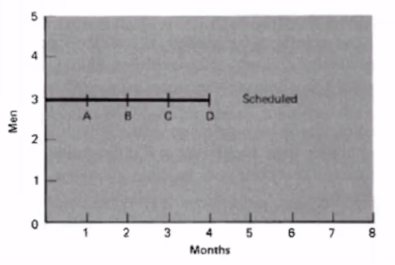
\includegraphics[width=\linewidth]{document/img/milestones.PNG}
		\caption{Milestone di progetto}
	\end{subfigure}
	\begin{subfigure}{.32 \textwidth}
		\centering
		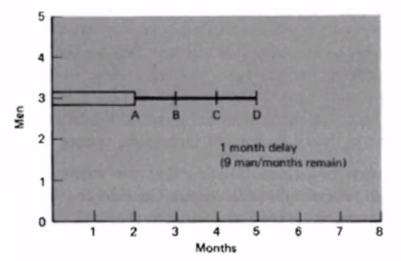
\includegraphics[width=\linewidth]{document/img/milestonelate.PNG}
		\caption{Milestone di progetto - Traslazione a causa del ritardo}
	\end{subfigure}
	\begin{subfigure}{.32 \textwidth}
		\centering
		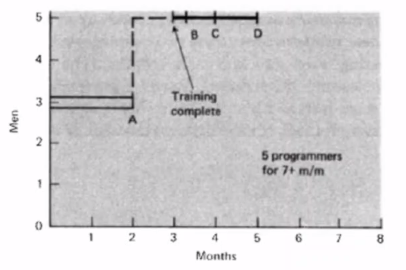
\includegraphics[width=\linewidth]{document/img/milestonepiuersonale.PNG}
		\caption{Milestone di progetto - Aumento personale}
	\end{subfigure}%
\end{figure}
\subsection{Gioie e Dolori}
Ora elencheremo alcuni motivi per cui si può essere felici di realizzare software. La leva deve essere molto forte su queste "gioie" perché la gente deve essere motivata.
\begin{itemize}
	\item La soddisfazione nel creare qualcosa;
	\item La soddisfazione nel creare qualcosa che gli altri useranno;
	\item La soddisfazione di risolvere un rompicapo complesso;
	\item Trovare stimoli per la propria curiosità;
	\item Lavorare con un mezzo molto flessibile;
\end{itemize}
Ci sono però anche dei dolori, e non sono pochi:
\begin{itemize}
	\item Necessità di estrema precisione;
	\item Mancanza di controllo in ciò che deve essere prodotto (molta dipendenza dalle specifiche);
	\item Dipendenza da altri programmi e/o programmatori;
	\item Il debug (scovare bug è difficile, a volte frustrante);
	\item A termine progetto il prodotto è spesso già obsoleto.
\end{itemize}
Nella gestione di un progetto è necessario tener conto sia degli aspetti positivi che di quelli negativi.
\subsection{Team}
Un elemento fondamentale per la buona riuscita del progetto è il Team. Il team deve essere composto correttamente, la composizione è fondamentale per una corretta gestione. Esistono diverse composizioni dei team, questi due sono solo esempi che è possibile seguire:
\begin{itemize}
	\item Esistono team più "tradizionali" che prevedono figure molto specializzate;
	\item Esistono team più "agili" dove sono presenti meno figure più "versatili".
\end{itemize}
\subsubsection{Surgical Team}
Il \textbf{Surgical Team}, adottato ancora oggi era molto più in voga intorno agli anni '90. Si tratta di un Team di persone di dimensioni limitate a cui vengono affidati dei task. Le figure presenti secondo l'inventore di questo approccio (Harlan Millis) sono le seguenti:
\begin{itemize}
	\item \textbf{Chirurgo}: dirige il team e prende tutte le decisioni sull'architettura e sulle specifiche. Testa il codice e scrive la documentazione;
	\item \textbf{Copilota}: è l'alter-ego del chirurgo, fa le stesse cose del Chirugo ma ha meno esperienza. Il suo parere può essere ignorato per dare priorità al Chirurgo;
	\item \textbf{Amministratore}: Esecutore delle direttive del Chirurgo. In genere questa figura è condivisa da più team;
	\item \textbf{Editor}: provvede a correggere, organizzare e aggiornare la documentazione scritta dal chirurgo;
	\item \textbf{Segretaria}: supporta l'amministrazione e l'editor, ma non deve avere conoscenze tecniche;
	\item \textbf{Program clerk}: supporta l'amministratore e l'editor, ma ha conoscenze e responsabilità tecniche;
	\item \textbf{Toolsmith}: realizza installa e mantiene tutti gli strumenti utili per gli sviluppatori;
	\item \textbf{Tester}: prepara ed esegue i test per i diversi casi d'uso;
	\item \textbf{Language lawyer}: si occupa di definire come usare il linguaggio di programmazione impiegato per l'implementazione di particolari parti di codice.
\end{itemize}
Al giorno d'oggi questa visione è vista come un po' rigida e datata. Molti di questi ruoli sono interpretati dalla stessa persona. La transizione tecnologica ha potenziato alcuni ruoli e nerfato altri. La tendenza degli ultimi anni è quella di avere team sempre più orizzonatali, in grado di ricoprire contemporaneamente più ruoli. Questo accade perché si risparmia molto tempo se si è in grado di "fare tutto". La divisione offerta da Millis anche se poco utilizzata oggi ha il pregio di riuscire a mostrare quali sono i ruoli in un team.
\subsubsection{Scrum Team}
Lo \textbf{Scrum Team}, in contrapposizione al Surgical Team, presenta meno figure ma più "versatili". Scrum è un Framework per lo sviluppo iterativo e incrementale dei prodotti software nato negli anni '90.\newline Il lavoro viene suddiviso in iterazioni dette \textbf{Sprint} che hanno una durata predeterminata e precisa. Esistono tre ruoli in uno Scrum Team:
\begin{itemize}
	\item \textbf{Product Owner}: ha la responsabilità sul prodotto. Se il prodotto non fa quello che ci si aspetta questa figura deve dialogare col cliente per rispondere alle sue esigenze. Non è responsabile del "come" vanno fatte le cose, ma del "cosa" bisogna fare;
	\item \textbf{Scrum Master}: non è il capo dello Scrum team, ma aiuta il team a crescere, fornisce indicazioni al team, orchestra il modo in cui vanno gestite le cose. Può anche essere una figura non tecnica;
	\item \textbf{Team di Sviluppo}: si tratta delle persone che hanno le competenze per raggiungere la soluzione del problema. Hanno la massima autonomia sulle scelte tecniche. Scrivono codice, documentazione e a volte fanno anche attività di segreteria.
\end{itemize}
La dimensione del team è un tema ancora piuttosto dibattuto:
Team troppo grandi non si riesco a gestire facilmente a causa dell'overhead delle comunicazioni. Essendo le comunicazioni molto frequenti nella metodologia scrum si rischia di perdere molto tempo.
Secondo Jeff Bezos un team deve avere un numero di componenti che possono essere sfamati da due pizze (Jeff Bezos' Two Pizza Team Rule).
\begin{warn}
	In America non capiscono proprio un cazzo di come si fa una pizza, e hanno un concetto diverso di sta cosa.
\end{warn}
Il numero ideale si aggira quindi intorno ai 4-8 sviluppatori. Il numero dipende anche dalla natura di ciò che si sta sviluppando. Il team può essere composto da \textit{generalisti} (sanno un po' di tutto, per esempio full-stack) o \textit{specialisti} (coprono uno specifico dominio), ma anche da un mix dei due.\newline
\subsection{Conceptual Integrity}
Il rispetto della \textbf{Conceptual Integrity} è molto importante. Per produrre un sistema efficace, efficiente e user friendly è necessario che sia rispettata la sua integrità concettuale, ossia è necessario che le funzionalità rispondano solo e solamente ai requisiti definiti in progettazione. Tutto ciò che non è definito e viene implementato è inutile ed è solo causa di perdita di tempo.
\begin{warn}
	MAI effettuare modifiche senza prima mettere mano ai requisiti!
\end{warn}
Necessario separare l'architettura dall'implementazione. Solo uno o due architetti decidono cosa sarà presente nel sistema e cosa no, ovviamente mantenendo centrale il bisogno dell'utente. Gli architetti definisicono il "cosa", mentre il resto del team pensa al "come". L'architetto può fare da \textit{collo di bottiglia} perché l'implementazione dipende dalle sue decisioni, ma una volta prese egli può delegare tranquillamente al team l'implementazione. Non dovrebbero fornire architetture troppo ricche e devono sempre tenere a mente i costi. Inoltre un architetto non dovrebbe essere estremamente specifico, in quanto il "come" va realizzato il sistema non spetta a lui. Sono gli sviluppatori che devono essere creativi e fornire le soluzioni adeguate in base alle richieste.\newline
Lo Scrum team è molto orizzontale e quindi molto democratico, al punto che anche il cliente "fa parte" del team di sviluppo. Uno degli equivoci più grandi è pensare che l'approccio Agile sia vicino all'anarchia e che i gradi di libertà siano troppi. Paradossalmente chi fa AGILE deve essere estremamente disciplinato per riuscire a gestire una catena orizzontale nel modo corretto.
\subsection{The Second-System Effect}
Non troppe persone sono d'accordo, specificando che il problema è molto più complesso di come affrontato da Brooks.
\begin{itemize}
	\item Il \textbf{primo sistema} che si progetta prevede solo le funzionalità richieste dall'utente.
	\item Il \textbf{secondo sistema} viene progettato aggiungendo tutto ciò che si ritiene sia stato dimenticato nel primo progetto. Bisogna stare attenti però ad arrivare ad un \textbf{better design} e non ad un \textbf{over design}, altrimenti avremo un impatto negativo sul rapporto costi/benefici.
\end{itemize}
Brooks consiglia di puntare sul personale che ha esperienza, o ancora meglio personale che conosce bene il problema, e che sono quindi in grado di evitarlo.
\subsection{Comunicazioni}
In quanti modi si può comunicare? Tanti:
\begin{itemize}
	\item \textbf{Informalmente}: telefonate, pause caffè, messaggistica, ad un pub... etc.\newline
	\textit{Vantaggi}:
	\begin{itemize}
		\item Molto veloce;
		\item Nel caso dell'istant messaging il tutto è asincrono, posso recuperare un'informazione senza necessariamente richiedere alla fonte.
	\end{itemize}
	\textit{Svantaggi}:
	\begin{itemize}
		\item Facile interpretare male un'informazione;
		\item Molta dispersione;
		\item Nessun tipo di strutturazione, soprattutto quando le informazioni sono tante.
	\end{itemize}
	\item \textbf{Meetings}: Riunioni a cadenza regolare o a bisogno dove il team informa sullo stato di avanzamento del progetto.\newline
	\textit{Vantaggi}:
	\begin{itemize}
		\item Redazione di un verbale che aiuta a tener traccia di ciò che si è detto.
	\end{itemize}
	\textit{Svantaggi}:
	\begin{itemize}
		\item Un verbale strutturato male è inutile perché è al pari di una comunicazione informale;
		\item La differenza tra meeting e comunicazione informale è molto labile, anche se è comunque più strutturata.
	\end{itemize}
	\item \textbf{Workbook}: Contenitore in cui sono riportati formalmente informazioni riguardanti il progetto. Ultimamente questa soluzione è molto adottata anche grazie a soluzioni cloud che hanno rimpiazzato il cartaceo.\newline
	\textit{Vantaggi}:
	\begin{itemize}
		\item Informazione integra e sempre sincronizzata per tutti.
	\end{itemize}
	\textit{Svantaggi}:
	\begin{itemize}
		\item Il lavoro di aggiornamento deve essere costante e spesso è un'operazione molto dispendiosa e noiosa.
	\end{itemize}
\end{itemize}
\subsection{Documentazione}
La documentazione è fondamentale perché:
\begin{itemize}
	\item indica il funzionamento di un programma, un componente, etc.;
	\item permette di ricordare cosa si è fatto a distanza di tempo;
	\item aiuta chi non ha realizzato il software a capirne il funzionamento;
	\item descrive formalmente le interfacce tra i componenti;
	\item aiuta a tenere traccia di problemi o a risolvere bugs;
	\item aiuta ai fini di testing;
	\item molti altri...
\end{itemize}
Le specifiche scritte dall'architetto possono essere fornite sotto forma di \textbf{Manuale}. Si tratta di uno strumento molto potente di design.\newline
Immaginiamo di avere il manuale di una macchinetta del caffè prima ancora che questa esista. Il manuale descrive perfettamente le funzionalità che questa deve avere e ci fornisce indicazioni precise su come portare avanti l'implementazione. Attraverso il manuale possiamo capire se i requisiti sono rispettati e possiamo capire se mancano informazioni (es: nel manuale non esiste il capitolo che spiega come ci si deve comportare nel caso in cui una cialda si incastri).\newline
Costruire il manuale è un ottimo modo per prototipare un prodotto senza nemmeno crearlo. Una volta finito il manuale si ha una buona base per iniziare a progettare, perché si hanno le idee molto chiare sul risultato. Se invece il team è ancora indeciso su alcuni aspetti è necessario rivedere il manuale per risolvere le criticità.\newline
A volte si può iniziare da un manuale più spoglio e arricchirlo mano a mano utilizzando un approccio simile all'AGILE.\newline
Brooks spiega le criticità della documentazione dicendo che "si perde tanto tempo a descrivere i rami e le foglie ma non si da l'idea di come è fatta la foresta".
\begin{info}[Esempio]
	Immaginiamo un sistema ERP. Descrivere nei minimi dettagli i singoli componenti del sistema è inutile se non si spiega correttamente come questi interagiscono tra loro.
\end{info}
Brooks individua i seguenti quesiti a cui è necessario dare una risposta:
\begin{itemize}
	\item \textbf{Purpose}: Qual è la funzione principale del software?
	\item \textbf{Environment}: Su quale macchina girerà il software? Quale sistema operativo? Quale configurazione?
	\item \textbf{Domain and Range}: Quale dominio di input è valido? Quale output è ammissibile e quale no?
	\item \textbf{Function Realized and Algorithm Used}: Cosa permette di fare il software e come?
	\item \textbf{Input-Output Formats}: Qual è il formato per poter effettuare input/output?
	\item \textbf{Operation Instruction}: Come si usa? Quali sono le eccezioni? Come vanno gestitw? Serve un corso per spiegare agli utenti come si usa? Il cliente può anche comprare il training oltre il software se necessario.
	\item \textbf{Options}: Che scelte può fare l'utente? Come gli viene permesso di compierle?
	\item \textbf{Running Time}: Quanto tempo impiega il software ad eseguire la funzionalità richiesta?
	\item \textbf{Accuracy and Checking}: Quanto è precisa la soluzione fornita dal software? Ci sono controlli aggiuntivi per verificare la correttezza?
\end{itemize}
La documentazione è utile perché i programmi devono essere modificati e/o corretti, quindi è necessario avere sempre a portata di mano i dettagli sulle implementazioni.\newline
Eventualmente è possibile anche elencare possibili miglioramenti che si possono effettuare, cosa può essere compatibile e cosa non ragionevole.\newline
Il codice stesso è documentazione. Un codice parlante non ha bisogno di troppa documentazione. L'unica controindicazione è che il codice va scritto in un certo modo. I nomi delle variabili, dei metodi etc. devono essere esplicativi. Utilizzare il codice come documentazione può semplificare notevolmente la vita anche quando una funzionalità è difficile da descrivere verbalmente. Esistono anche tool per generare documentazione a partire dal codice o viceversa.

\noindent Per gestire un progetto è necessario quantomeno produrre la seguente documentazione:
\begin{itemize}
	\item \textbf{What(objective)}: Un documento che specifica quali sono gli obiettivi, i vincoli, le priorità;
	\item \textbf{What(product specifications)}: La prima versione può essere una proposta molto sintetica che va via via evolvendosi, diventando sempre più simile ad un manuale;
	\item \textbf{When (schedule)}: Qui c'è tanto lavoro da fare: di solito questo non è un solo documento ma un insieme di documenti. Bisogna pianificare le attività di progetto (per esempio utilizzando GANTT) o strumenti software specifici;
	\item \textbf{How Much (budget)}: Un documento che specifica come utilizzare il budget. Influenza pesantemente anche le scelte tecniche;
	\item \textbf{Where (space allocation)}: Nel caso del software non è un tema fondamentale, ma non deve essere sottovalutato il "dove" un software viene discusso/progettato. Ci sono disposizioni da rispettare anche nel caso di sviluppo davanti ad un PC;
	\item \textbf{Who}: Estremamente importante. Descrive le risorse umane coinvolte nel progetto, si sceglie quali sono le responsabilità per stabilire i ruoli etc.
\end{itemize}
Perché è importante avere documentazione formale?
\begin{itemize}
	\item \textbf{Mettere per iscritto è fondamentale}: Può aiutare a capire meglio se si sono dimenticati dei pezzi fondamentali e aiuta a far capire quali decisioni sono state prese e perché.
	\item \textbf{La documentazione aiuta a comunicare quali decisione sono state prese}: Alcune persone che prenderanno parte al progetto probabilmente non hanno fatto parte della riunione che ha portato a scrivere il documento e avranno bisogno di recuperare.
	\item \textbf{La documentazione è una base di dati in formato di checklist che aiuta a capire cosa serve per realizzare il progetto}: Deve essere scritta in modo tale che sia utile. La documentazione va aggiornata quando cambiano i requisiti. La documentazione deve essere un documento che aiuta a rendere il lavoro più "rilassante" e semplice da eseguire.
	\subsection{La rivoluzione Agile}
	\subsubsection{Agile Manifesto}
	Com'è nato il manifesto Agile? Nel 2001 17 sviluppatori si incontrano per cercare di ideare metodologie di lavoro "leggere". Non andò benissimo ma nacque comunque il Manifesto for Agile Software Development. Non tutti ebbero le stesse idee, ma ci fu accordo su quattro punti.
	\begin{info}[MANIFESTO]
		\newline We are uncovering better ways of developing
		software by doing it and helping others do it.\newline
		Through this work we have come to value:
		\begin{itemize}
			\item \textcolor{red}{Individuals and interactions} over processes and tools;
			\item \textcolor{red}{Working software} over comprehensive documentation;
			\item \textcolor{red}{Customer collaboration} over contract negotiation;
			\item \textcolor{red}{Responding to change} over following a plan;
		\end{itemize}
		That is, while there is value in the items on
		the right, we value the items on the left more.
	\end{info}
	Da questo documento possiamo trarre delle considerazioni:\newline
	Sia ciò che è rosso sia ciò che è nero è importante, ma ciò che è rosso lo è di più. Per esempio processi e i tool sono importanti, ma è ancora più importante l'individuo e la comunicazione con gli altri. Questo significa per esempio che non tutto potrebbe essere chiaro, magari soprattutto all'inizio, e che quindi è sì, importante portare avanti i processi, ma solo se la comunicazione è stata efficace.\newline
	La documentazione è molto importante, può essere estremamente completa, ma ancora più importante è che il codice giri. Se il software non funziona una documentazione completa è inutile per il cliente.\newline
	Generalmente si stabilisce con il cliente cosa mettere nel contratto. Se il sistema risulta lento ma nel contratto non ci sono vincoli a riguardo il dev è legalmente a posto. Quello che invece richiede Agile è la collaborazione con il cliente. Richiesta la flessibilità di rivedere il capitolato in corso d'opera per andare incontro ai bisogni del cliente. Questo ha un costo, ma stilando il contratto anche questo aspetto è tenuto da conto e viene illustrato al cliente, che solitamente avrà comunque il piacere di pagare un po' di più per vedere rispettati i suoi bisogni.\newline
	Seguire un piano è importante e va rispettato, ma bisogna rispondere al cambiamento. Il metodo Agile non intende non stilare un piano "perché tanto cambierà e quindi si perde solo tempo". Il punto è stilare un piano, ma farlo in modo da poter avere la flessibilità di modificarlo in corso d'opera.
\end{itemize}
\subsubsection{Principi del Software Agile}
Seguono i 12 principi del Software Agile:
\begin{itemize}
	\item La priorità più alta per avere un cliente contento consiste nel donargli del software funzionante ad intervalli di tempo regolari. Questo deve accadere perché in questo modo gli utenti acquisiscono fiducia nei dev. Gli utenti utilizzando il software capiscono cosa non va bene e lo notificano in modo da "aggiustare il tiro" il prima possibile. In un approccio a cascata gestire un cambiamento è molto più difficile e soprattutto molto più costoso.
	\item Ben venga il cambiamento, anche se in ritardo. Il processo agile considera il cambiamento come un'opportunità importante per il cliente per dare un vantaggio competitivo. Intervenire nel progetto in corso d'opera per aggiungere funzionalità che sono presenti in software di aziende rivali è un ottimo modo per mantenere la rivalità e forse anche sorpassarla.
	\item Consegnare dei risultati dopo una certa scadenza, ad intervalli regolari. In questo modo gli sviluppatori sono più invogliati a raggiungere gli obiettivi e riescono ad organizzarsi per il meglio.
	\item Non è solo compito degli sviluppatori fornire una soluzione informatica. Il risultato deve essere frutto di un lavoro condiviso da tutti i tipi di figure che lavoreranno insieme ogni giorno.
	\item Le persone sono importanti, mai sminuirle. Importante avere fiducia e delegare compiti ad altri. La fiducia è centrale e il risultato deve essere raggiunto anche grazie all'ambiente di lavoro che deve rendere contenti ed invogliare i dev. Uno dei pericoli più grandi è l'abbandono del progetto da parte di qualcuno lungo la strada.
	\item Il modo migliore e più efficiente per comunicare è la face-to-face conversation (comunicazione informale). Non deve essere l'unico metodo di comunicazione ma è quello più indicato nelle normali giornate di lavoro in cui serve solo risolvere qualche incertezza minore.
	\item Il software funzionante è la misura di progresso principale. Se ci sono 4 su 10 funzionalità che il software rispetta allora il software è pronto circa al 40\%.
	\item Bisogna lavorare in modo che sia possibile lavorare sempre alla stessa velocità (e non solo lavorare alla stessa velocità). Questo significa evitare il più possibile il debito tecnico, altrimenti le cose si faranno sempre più complicate. I clienti chiederanno cambiamenti. Lo sviluppo deve essere sostenibile, se introdurre un cambiamento è difficile e porta paura nei dev qualcosa è andato storto. Il livello di difficoltà nell'applicare modifiche deve rimanere costante.
	\item L'attenzione all'eccellenza tecnica e ad un buon design incentiva l'agilità. Più qualcosa è fatto bene, meno problemi ci saranno da risolvere e più facile sarà apportare i cambiamenti. Utilizzare pattern aiuta ad arrivare allo stato dell'arte.
	\item La semplicità è essenziale. Bisogna massimizzare il lavoro che non deve essere fatto. Bisogna aggiungere solo codice che aiuta a raggiungere un requisito. Tutto quel che viene aggiunto che non contribuisce a farlo complica solo le cose e soprattutto costa. Se si pensa che qualcosa è utile bisogna prima chiedere al cliente se ne necessita, e nel caso rivalutare i requisiti.
	\item Il product owner dice cosa deve essere fatto, il team di sviluppo decide come fare in autonomia, senza colli di bottiglia con l'architetto o altre autorità. Ancora una volta il focus è sulla delegazione, sulla fiducia nel team, sul miglioramento continuo.
	\item A intervalli regolari il team deve riflettere su come migliorare.
\end{itemize}
Il movimento Agile non è anti-metodologia. Bisogna trovare il giusto bilanciamento tra ciò che bisogna fare per gestire il progetto e ciò che non bisogna fare.
L'agile è a favore della documentazione, ma a sfavore di tomi di documentazioni inutile perché non mantenuti aggiornati o con troppo contenuto informativo.\newline
La pianificazione ha un limite. Prima o poi è necessario convergere verso un "prodotto finale". Allo stesso modo è importante anche apportare cambiamenti dove necessario e non essere troppo rigidi coi piani. Anche la flessibilità ha un limite, non è possibile stravolgere completamente un progetto grazie all'approccio Agile.
